% Options for packages loaded elsewhere
\PassOptionsToPackage{unicode}{hyperref}
\PassOptionsToPackage{hyphens}{url}
\PassOptionsToPackage{dvipsnames,svgnames,x11names}{xcolor}
%
\documentclass[
  12pt]{article}

\usepackage{amsmath,amssymb}
\usepackage{iftex}
\ifPDFTeX
  \usepackage[T1]{fontenc}
  \usepackage[utf8]{inputenc}
  \usepackage{textcomp} % provide euro and other symbols
\else % if luatex or xetex
  \usepackage{unicode-math}
  \defaultfontfeatures{Scale=MatchLowercase}
  \defaultfontfeatures[\rmfamily]{Ligatures=TeX,Scale=1}
\fi
\usepackage{lmodern}
\ifPDFTeX\else  
    % xetex/luatex font selection
\fi
% Use upquote if available, for straight quotes in verbatim environments
\IfFileExists{upquote.sty}{\usepackage{upquote}}{}
\IfFileExists{microtype.sty}{% use microtype if available
  \usepackage[]{microtype}
  \UseMicrotypeSet[protrusion]{basicmath} % disable protrusion for tt fonts
}{}
\makeatletter
\@ifundefined{KOMAClassName}{% if non-KOMA class
  \IfFileExists{parskip.sty}{%
    \usepackage{parskip}
  }{% else
    \setlength{\parindent}{0pt}
    \setlength{\parskip}{6pt plus 2pt minus 1pt}}
}{% if KOMA class
  \KOMAoptions{parskip=half}}
\makeatother
\usepackage{xcolor}
\setlength{\emergencystretch}{3em} % prevent overfull lines
\setcounter{secnumdepth}{5}
% Make \paragraph and \subparagraph free-standing
\ifx\paragraph\undefined\else
  \let\oldparagraph\paragraph
  \renewcommand{\paragraph}[1]{\oldparagraph{#1}\mbox{}}
\fi
\ifx\subparagraph\undefined\else
  \let\oldsubparagraph\subparagraph
  \renewcommand{\subparagraph}[1]{\oldsubparagraph{#1}\mbox{}}
\fi


\providecommand{\tightlist}{%
  \setlength{\itemsep}{0pt}\setlength{\parskip}{0pt}}\usepackage{longtable,booktabs,array}
\usepackage{calc} % for calculating minipage widths
% Correct order of tables after \paragraph or \subparagraph
\usepackage{etoolbox}
\makeatletter
\patchcmd\longtable{\par}{\if@noskipsec\mbox{}\fi\par}{}{}
\makeatother
% Allow footnotes in longtable head/foot
\IfFileExists{footnotehyper.sty}{\usepackage{footnotehyper}}{\usepackage{footnote}}
\makesavenoteenv{longtable}
\usepackage{graphicx}
\makeatletter
\def\maxwidth{\ifdim\Gin@nat@width>\linewidth\linewidth\else\Gin@nat@width\fi}
\def\maxheight{\ifdim\Gin@nat@height>\textheight\textheight\else\Gin@nat@height\fi}
\makeatother
% Scale images if necessary, so that they will not overflow the page
% margins by default, and it is still possible to overwrite the defaults
% using explicit options in \includegraphics[width, height, ...]{}
\setkeys{Gin}{width=\maxwidth,height=\maxheight,keepaspectratio}
% Set default figure placement to htbp
\makeatletter
\def\fps@figure{htbp}
\makeatother

\addtolength{\oddsidemargin}{-.5in}%
\addtolength{\evensidemargin}{-1in}%
\addtolength{\textwidth}{1in}%
\addtolength{\textheight}{1.7in}%
\addtolength{\topmargin}{-1in}%

\makeatletter
\makeatother
\makeatletter
\makeatother
\makeatletter
\@ifpackageloaded{caption}{}{\usepackage{caption}}
\AtBeginDocument{%
\ifdefined\contentsname
  \renewcommand*\contentsname{Table of contents}
\else
  \newcommand\contentsname{Table of contents}
\fi
\ifdefined\listfigurename
  \renewcommand*\listfigurename{List of Figures}
\else
  \newcommand\listfigurename{List of Figures}
\fi
\ifdefined\listtablename
  \renewcommand*\listtablename{List of Tables}
\else
  \newcommand\listtablename{List of Tables}
\fi
\ifdefined\figurename
  \renewcommand*\figurename{Figure}
\else
  \newcommand\figurename{Figure}
\fi
\ifdefined\tablename
  \renewcommand*\tablename{Table}
\else
  \newcommand\tablename{Table}
\fi
}
\@ifpackageloaded{float}{}{\usepackage{float}}
\floatstyle{ruled}
\@ifundefined{c@chapter}{\newfloat{codelisting}{h}{lop}}{\newfloat{codelisting}{h}{lop}[chapter]}
\floatname{codelisting}{Listing}
\newcommand*\listoflistings{\listof{codelisting}{List of Listings}}
\makeatother
\makeatletter
\@ifpackageloaded{caption}{}{\usepackage{caption}}
\@ifpackageloaded{subcaption}{}{\usepackage{subcaption}}
\makeatother
\makeatletter
\@ifpackageloaded{tcolorbox}{}{\usepackage[skins,breakable]{tcolorbox}}
\makeatother
\makeatletter
\@ifundefined{shadecolor}{\definecolor{shadecolor}{rgb}{.97, .97, .97}}
\makeatother
\makeatletter
\makeatother
\makeatletter
\makeatother
\ifLuaTeX
  \usepackage{selnolig}  % disable illegal ligatures
\fi
\usepackage[]{natbib}
\bibliographystyle{agsm}
\IfFileExists{bookmark.sty}{\usepackage{bookmark}}{\usepackage{hyperref}}
\IfFileExists{xurl.sty}{\usepackage{xurl}}{} % add URL line breaks if available
\urlstyle{same} % disable monospaced font for URLs
\hypersetup{
  pdftitle={Appendix: Visualising How Non-linear Dimension Reduction Warps Your Data},
  pdfauthor={Jayani P.G. Lakshika; Dianne Cook; Paul Harrison; Michael Lydeamore; Thiyanga S. Talagala},
  colorlinks=true,
  linkcolor={blue},
  filecolor={Maroon},
  citecolor={Blue},
  urlcolor={Blue},
  pdfcreator={LaTeX via pandoc}}


\begin{document}


\def\spacingset#1{\renewcommand{\baselinestretch}%
{#1}\small\normalsize} \spacingset{1}

%%%%%%%%%%%%%%%%%%%%%%%%%%%%%%%%%%%%%%%%%%%%%%%%%%%%%%%%%%%%%%%%%%%%%%%%%%%%%%

\title{\bf Appendix: Visualising How Non-linear Dimension Reduction
Warps Your Data}
\author{
Jayani P.G. Lakshika\\
Econometrics \& Business Statistics, Monash University\\
and\\Dianne Cook\\
Econometrics \& Business Statistics, Monash University\\
and\\Paul Harrison\\
MGBP, BDInstitute, Monash University\\
and\\Michael Lydeamore\\
Econometrics \& Business Statistics, Monash University\\
and\\Thiyanga S. Talagala\\
Statistics, University of Sri Jayewardenepura\\
}
\maketitle

\bigskip
\bigskip
\begin{abstract}

\end{abstract}


\newpage
\spacingset{1} % DON'T change the spacing! (Default 1.9)

\ifdefined\Shaded\renewenvironment{Shaded}{\begin{tcolorbox}[frame hidden, interior hidden, borderline west={3pt}{0pt}{shadecolor}, sharp corners, boxrule=0pt, breakable, enhanced]}{\end{tcolorbox}}\fi

Paramter tunning

\hypertarget{total-number-of-bins}{%
\section{Total number of bins}\label{total-number-of-bins}}

The total number of bins represents the overall count of hexagonal bins
within the hexagonal grid. This count is determined by multiplying the
number of bins along the x-axis (\(b_1\)) with the number of bins along
the y-axis (\(b_2\)), according to the formula:

\begin{equation}\protect\hypertarget{eq-equationp1}{}{
 b = b_1 \times b_2
}\label{eq-equationp1}\end{equation}

Here, \(b\) denotes the total number of bins. By adjusting the parameter
\(b_1\), we have control over the total number of bins (\(b\)). Hence,
fine-tuning \(b_1\) enables us to customize and optimize the total bin
count based on the desired configuration along the x-axis.

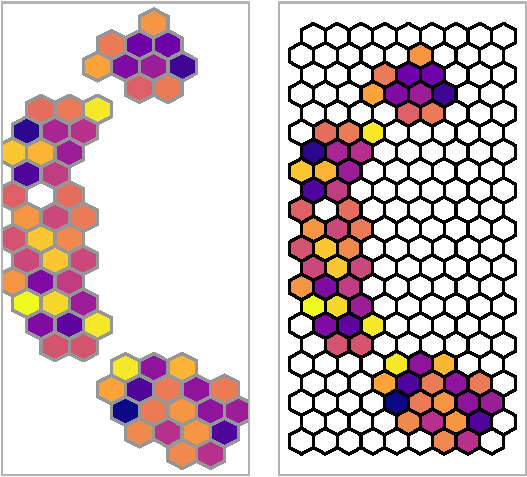
\includegraphics[width=1\textwidth,height=\textheight]{appendix_files/figure-pdf/unnamed-chunk-9-1.pdf}

\hypertarget{benchmark-value-to-remove-low-density-hexagons}{%
\section{Benchmark value to remove low-density
hexagons}\label{benchmark-value-to-remove-low-density-hexagons}}

In the step of addressing low-density hexagons, which can arise from
sparsely represented data in certain regions, we employ a systematic
strategy. The goal is to ensure a more comprehensive coverage of the
data by removing hexagons with low data density. To achieve this, we
initiate the process by identifying, for each hex bin, the six nearest
hex bins based on an equal 2D distance metric. Following this, we
calculate the mean density (see Equation~\ref{eq-equationp3}), as
outlined in the equation:

\begin{equation}\protect\hypertarget{eq-equationp2}{}{
 \text{standard count} = \frac{\text{count}}{\text{max count}}
}\label{eq-equationp2}\end{equation}

\begin{equation}\protect\hypertarget{eq-equationp3}{}{
 \text{mean density} = \frac{\text{standard count}}{6}
}\label{eq-equationp3}\end{equation}

The standard count is derived from the number of observations in the hex
bins (see Equation~\ref{eq-equationp2}). Next, we examine the
distribution of mean densities across all hex bins and designate the
first quartile as the benchmark value for removing low-density hexagons.
Finally, hex bins with mean densities below this benchmark value are
removed from consideration. This meticulous procedure ensures the
elimination of regions with inadequate data density, allowing the focus
to shift to areas with more significant data representation. The result
is the preservation of the overall structure of the data in the
low-dimensional space, as illustrated in \textbf{?@fig-bintorm} (c).

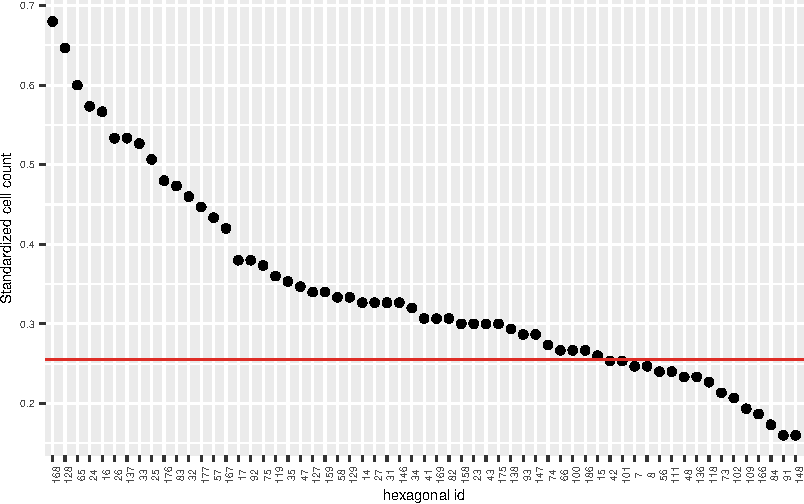
\includegraphics{appendix_files/figure-pdf/unnamed-chunk-14-1.pdf}

\begin{verbatim}
Joining with `by = join_by(hexID)`
\end{verbatim}

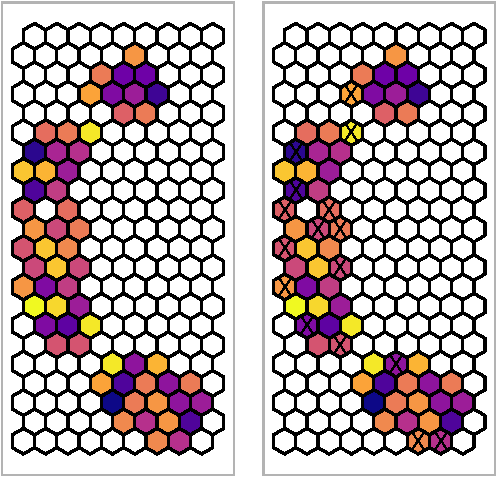
\includegraphics{appendix_files/figure-pdf/unnamed-chunk-15-1.pdf}

\hypertarget{benchmark-value-to-remove-long-edges}{%
\section{Benchmark value to remove long
edges}\label{benchmark-value-to-remove-long-edges}}

In this step, we aim to create a smoother surface in the low-dimensional
space by removing long edges from the triangular mesh. This process
helps eliminate outliers and noise while preserving important local
relationships and intricate structures within the data. To achieve this,
distances between vertices are sorted, and unique distance values are
extracted. A data frame is created to calculate the differences between
consecutive distance values, and the largest difference serves as a
threshold to identify long edges. By removing edges that exceed this
threshold, the algorithm refines the triangular mesh (see
\textbf{?@fig-traingularmeshgr}).

\begin{figure}

{\centering 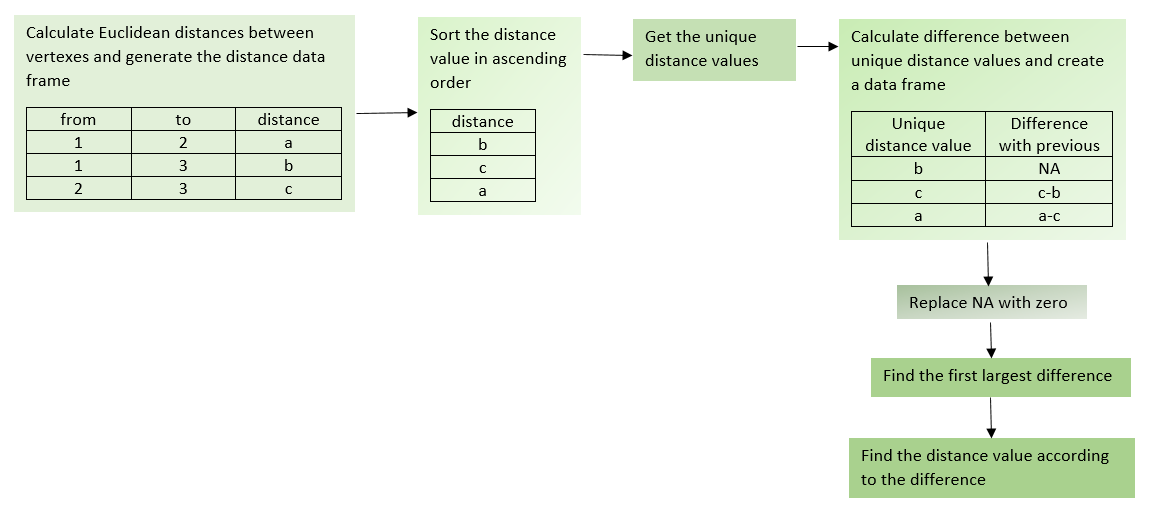
\includegraphics[width=1\textwidth,height=1\textheight]{figures/remove_long_edges_workflow.png}

}

\caption{\label{fig-rmlgmeth}A flow diagram detailing the steps taken to
find the benchmark value to remove long edges.}

\end{figure}

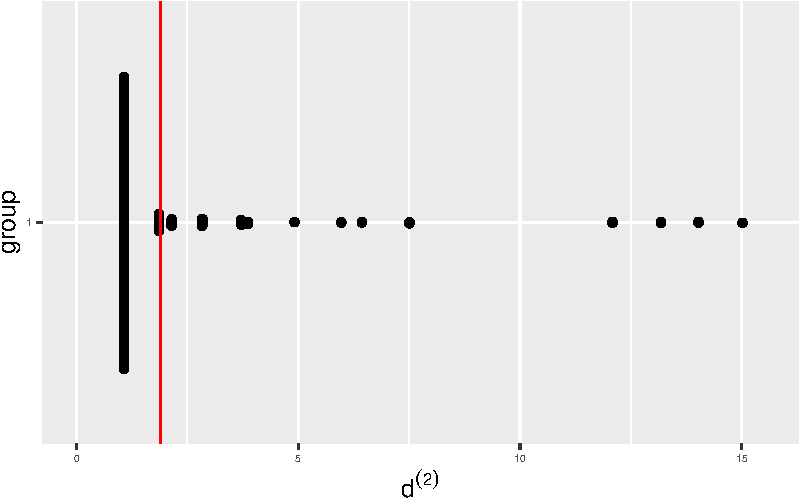
\includegraphics{appendix_files/figure-pdf/unnamed-chunk-16-1.pdf}

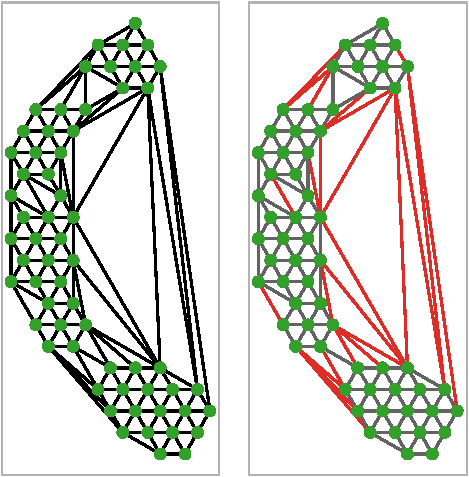
\includegraphics{appendix_files/figure-pdf/unnamed-chunk-17-1.pdf}



\end{document}
